\documentclass[a4paper,UTF8]{article}
\usepackage{ctex}
\usepackage[margin=1.25in]{geometry}
\usepackage{color}
\usepackage{graphicx}
\usepackage{amssymb}
\usepackage{amsmath}
\usepackage{amsthm}
\usepackage{enumerate}
\usepackage{bm}
\usepackage{hyperref}
\usepackage{pgfplots}
\usepackage{epsfig}
\usepackage{color}
\usepackage{tcolorbox}
\usepackage{mdframed}
\usepackage{lipsum}
\usepackage{natbib}
\usepackage{float}
\newmdtheoremenv{thm-box}{myThm}
\newmdtheoremenv{prop-box}{Proposition}
\newmdtheoremenv{def-box}{定义}

\setlength{\evensidemargin}{.25in}
\setlength{\textwidth}{6in}
\setlength{\topmargin}{-0.5in}
\setlength{\topmargin}{-0.5in}
% \setlength{\textheight}{9.5in}
%%%%%%%%%%%%%%%%%%此处用于设置页眉页脚%%%%%%%%%%%%%%%%%%
\usepackage{fancyhdr}                                
\usepackage{lastpage}                                   
\usepackage{layout}                                     
\newtheorem*{solution}{Solution}

\footskip = 10pt 
\pagestyle{fancy}                    % 设置页眉                 
\lhead{2020年秋季}                    
\chead{高级机器学习}                                                
% \rhead{第\thepage/\pageref{LastPage}页} 
\rhead{作业二}                                                                                               
\cfoot{\thepage}                                                
\renewcommand{\headrulewidth}{1pt}  			%页眉线宽,设为0可以去页眉线
\setlength{\skip\footins}{0.5cm}    			%脚注与正文的距离           
\renewcommand{\footrulewidth}{0pt}  			%页脚线宽,设为0可以去页脚线

\makeatletter 									%设置双线页眉                                        
\def\headrule{{\if@fancyplain\let\headrulewidth\plainheadrulewidth\fi%
\hrule\@height 1.0pt \@width\headwidth\vskip1pt	%上面线为1pt粗  
\hrule\@height 0.5pt\@width\headwidth  			%下面0.5pt粗            
\vskip-2\headrulewidth\vskip-1pt}      			%两条线的距离1pt        
 \vspace{6mm}}     								%双线与下面正文之间的垂直间距              
\makeatother  

%%%%%%%%%%%%%%%%%%%%%%%%%%%%%%%%%%%%%%%%%%%%%%
\numberwithin{equation}{section}
%\usepackage[thmmarks, amsmath, thref]{ntheorem}
\newtheorem{myThm}{myThm}
\newtheorem*{myDef}{Definition}
\newtheorem*{mySol}{Solution}
\newtheorem*{myProof}{Proof}
\newtheorem*{myRemark}{备注}
\renewcommand{\tilde}{\widetilde}
\renewcommand{\hat}{\widehat}
\newcommand{\indep}{\rotatebox[origin=c]{90}{$\models$}}
\newcommand*\diff{\mathop{}\!\mathrm{d}}

\usepackage{multirow}

%--

%--
\begin{document}
\title{高级机器学习\\
大作业}
\author{高辰潇\, 181220014} 
\maketitle
%%%%%%%% 注意: 使用XeLatex 编译可能会报错,请使用 pdfLaTex 编译 %%%%%%%


\newpage
\section{Introduction}
本次的作业为使用条件随机场(conditional random field,CRF)解决OCR(optical character recognition)问题。

在CRF模型中,有两种变量:我们要建模的隐藏变量和始终观察到的变量。对于OCR,我们要在观察的字符图像(也就是每个图像对应的像素数组)的情况下,对字符(例如“a”或“c”)进行建模。通常来说,未观察到的变量用$Y$表示,观察到的变量用$X$表示。CRF试图对$P(Y|X)$建模,即给定观察到的图像上字符的条件分布。该模型的结构如\ref{Fig.main1}下所示:
\begin{figure}[h] 
\centering
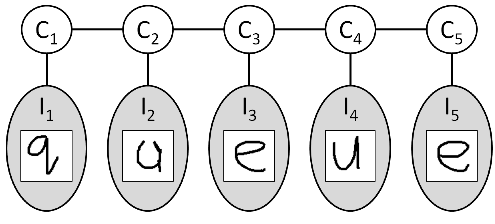
\includegraphics[width=0.7\textwidth]{figs/fig0.png} 
\caption{Markov Network} 
\label{Fig.main1}
\end{figure}

在CRF中,每个特征都对应一个权重$\theta_i$,在给定特征和权重的情况下,条件概率分布可以表示为:
\begin{equation}
P(\mathbf{Y} \mid \mathbf{x}: \theta)=\frac{1}{Z_{\mathbf{x}}(\theta)} \exp \left\{\sum_{i=1}^{k} \theta_{i} f_{i}\left(\mathbf{Y}, \mathbf{x}\right)\right\}\label{eq1}
\end{equation}

其中,$Z_x(\theta)$为配方函数
\begin{equation}
Z_{\mathbf{x}}(\theta) \equiv \sum_{\mathbf{Y}} \exp \left\{\sum_{i=1}^{k} \theta_{i} f_{i}\left(\mathbf{Y}, \mathbf{x}\right)\right\}
\end{equation}

在这次的任务中,一共有三类特征,三类特征均为指示函数,即满足条件时$f=1$,不满足时$f=0$:
\begin{itemize}
    \item $f_{i, c}^{C}\left(Y_{i}\right)$,指示是否$Y_i = c$
    \item $f_{i, j, c, d}^{I}\left(Y_{i}, x_{i j}\right)$,指示是否$Y_i=c,x_{ij}=d$
    \item $f_{i, c, d}^{P}\left(Y_{i}, Y_{i+1}\right)$,指示是否$Y_i=c,Y_{i+1}=d$
\end{itemize}

建立好模型,给定训练样本,我们就可以使用最大似然估计来进行学习:
\begin{equation}
    LL(\mathbf{x},\mathbf{Y},\theta) =\sum_{i=1}^{k} \theta_{i} f_{i}(\mathbf{Y}, \mathbf{x}) -\log \left(Z_{\mathbf{x}}(\theta)\right)\label{eq2}
\end{equation}

对于这个目标,我们可以使用梯度上升算法学习参数。

\section{Dataset}
本题中的数据集一共包含两个部分\texttt{trainset}和\texttt{testset}, 分别是训练集和测试集.训练集中有400个样本,测试集中有200个样本. 每个样本被存储在一个\texttt{txt}文件中, 第一行为对应的单词, 之后的每行为单词的每个字母对应的像素的状态.

\section{Assignment}
\begin{enumerate}
    \item 建立CRF模型,在训练集上进行训练,使用梯度上升的方法对模型参数进行求解,即求解公式\eqref{eq2}(注:不允许使用现有的CRF包,使用python实现)。
    \item 在模型训练完成后,在测试集上进行推断,评价模型的性能。
    \item 使用一些其他方法提高模型性能,可参考以下几个方面但不限于此:
    \begin{itemize}
        \item 提高模型表达能力:如在CRF图上添加新的连接。
        \item 缓解模型过拟合:如添加正则项。
        \item 加速模型训练过程:如权重共享。
    \end{itemize}
    \item 完成实验报告,主要包含具体的实现方法,如何复现运行代码,对模型的改进以及结果的分析等部分。
\end{enumerate}
\section {实验报告}

\subsection{算法描述}
\par 接下来的推导中,数学符号的定义均基于《统计学习方法》11.2.3中的符号定义。具体而言,我们将所有的特征及其权值使用统一的符号表示,分别记为$f_k(y_{i-1}, y_i, x, i)$和$w_k$,其中$k=1,2,3,...,K$。
\par 由此定义全局特征向量$F(y, x)$和权重向量$w$
$$F(y, x)=\left(f_1(y, x), f_2(y, x), ...,f_K(y, x)\right)^\top$$
$$w=\left(w_1, w_2, ..., w_K\right)^\top$$
于是条件随机场可表示为如下简化形式
$$
\begin{aligned}
    P(y|x)=&=\frac 1{Z(x)}\exp(w^\top F(y, x))\\
    Z(x)&=\sum_{y'}\exp(w^\top F(y', x))
\end{aligned}
$$
\subsubsection{对数似然与梯度}
\par 给定数据集$\mathcal{D}=\{(x^{1}, y^{1}), ..., (x^{j}, y^{j}), ...(x^{J}, y^{J})\}$,对数似然函数为
\begin{equation}\label{eq0}
\begin{aligned}
    LL(\mathcal{D})&= \log \prod_{j=1}^J P(y^{j}|x^{j})\\
    &=\sum_{j=1}^Jw^\top F(y^{j}, x^{j})-\log Z(x^{j})\\
\end{aligned}
\end{equation}
对参数$w$求导,得到
\begin{equation}\label{eq1}
\begin{aligned}
    \frac {\partial LL(\mathcal{D})}{\partial w} &= \sum_{j=1}^J\left(F(y^j, x^j)-\frac 1{Z(x^j)}\frac {\partial Z(x^j)}{\partial w}\right)\\
    &=\sum_{j=1}^J\left(F(y^j, x^j)-\frac 1{Z(x^j)}\sum_{y'}\exp(w^\top F(y', x^j))F(y', x^j)\right)\\
    &=\sum_{j=1}^J\left(F(y^j, x^j)-\sum_{y'}P(y'|x^j)F(y', x^j)\right)\\
    &=\sum_{j=1}^J\left(F(y^j, x^j)-\mathbb{E}_{y'\sim P(y'|x^j)}\left[F(y', x^j)\right]\right)\\
\end{aligned}
\end{equation}
\par 从(\ref{eq1})可以看出,对数似然对参数$w$的导数的方向,与样本特征函数与其特征函数期望之差的方向相同。在使用梯度上升算法对梯度进行更新后,特征函数的期望$\mathbb{E}_{y'\sim P(y'|x^j)}\left[F(y', x^j)\right]$会向$F(y^j, x^j)$靠近。

\subsubsection{学习算法}
\par 我使用的是梯度上升算法对参数$w$进行优化。参数学习算法分为两个步骤,第一步是求解对数似然,第二步是计算梯度。
\begin{enumerate}
    \item \par\textbf{求解对数似然}
        \par 求解对数似然部分我使用的是《统计学习方法》一书11.3.1章的前向后向算法。假设序列长度为$n$,该算法首先需要计算概率矩阵$M_i, i=1, 2, ..., n+1$,然后定义前向向量$\alpha_i(\cdot|x)$,其第$i$个元素表示位置$i$的标记是$y_i$并且从$1$到$i$的前部分标记序列的非规范化概率。基于动态规划算法,可使用迭代式$\alpha^\top_i(\cdot|x)=\alpha^\top_{i-1} (\cdot|x)M_i$计算得到最后一个位置的前向向量$\alpha_n(\cdot|x)$。此时规范化因子可通过$Z(x)=\mathbf{1}^\top \alpha_n(\cdot|x)$求得。
        
        \par 求得$Z(x)$后,代入式(\ref{eq0})即可得到对数似然函数。
    \item \par\textbf{计算梯度}
        
    \par 式(\ref{eq1})给出了一个求解梯度的计算式,但是式中需要对所有可能的$y'$进行遍历,这一操作的复杂度随序列长度成指数型增长。我在实际实现时使用了pytorch对参数$w$进行自动微分。
\end{enumerate}

\subsubsection{模型解码}
\par 在求解得到模型参数后,可使用维特比算法求解给定观察$x$的最可能状态序列$y^*$。
\par 这里用到的维特比算法与《统计学习方法》231-233页叙述的内容完全一致,在此仅作简要描述。
\par 定义维特比变量$\delta_i(l)$和备忘录变量$\Phi_i(l)$为
$$
\begin{aligned}
    \delta_i(l)=\max_{1\leq j\leq m}\{\delta_{i-1}(j)+w^\top F_i(y_{i-1}=j, y_i=l, x)\}\quad\quad l=1,2,...,m\\
    \Phi_i(l) = \arg\max \{\delta_{i-1}(j)+w^\top F_i(y_{i-1}=j, y_i=l, x)\}\quad\quad l=1,2,...,m\\
\end{aligned}
$$
分别表示从第一个位置到位置$i$的各个标记$l=1,2,...,m$的非规范化概率的最大值和最大值路径。易见维特比变量可使用动态规划算法进行迭代求解。
\par 求得最后一个位置的维特比变量后,只需根据最大的概率值回溯路径即可得到最可能路径。


\subsection{代码实现}
\subsubsection{代码结构与运行方式}
\begin{itemize}
    \item src目录中包含三个.py文件,其中utils.py定义数据加载相关的函数;feature\_functions.py实现了三种特征函数,并为它们实现了统一的调用接口;CRF.py为主要模块,其中定义了用于实现OCR识别的类CRF\_OCR。
    \item \textbf{运行方式}为:在根目录下,执行命令 python3 src/CRF.py,即可开始加载数据集、训练并在测试集上进行测试。
\end{itemize}

\subsubsection{关键部分}
\begin{itemize}
    \item 本项目基于pytorch框架,使用neg-loglikelyhood损失对模型参数$w$进行优化。
    \item 在实现时,为第一节中提到的三种特征函数实现了统一的调用接口。
    \item 训练的pipeline为:
    \begin{enumerate}
        \item 根据输入数据$X$(像素点)和特征函数簇,计算特征矩阵,形状为$(l, m, m, K)$。其中$l$为序列长度,$m$为标签种类数,$K$为特征函数个数。
        \item CRF.forward()部分,将特征矩阵与模型参数$w$作点乘,得到概率矩阵$M_i, \quad i=1,2,...,l$。此处概率矩阵定义见本报告的4.1.2节和《统计学习方法》一书的11.2.4节。值得注意的是,为了防止指数上溢,这里矩阵的元素均为原来的对数。
        \item 根据概率矩阵计算前向向量$\alpha$和对数似然函数,并取负作为损失函数。
        \item 根据损失函数反向传播误差,进行一次梯度更新。
    \end{enumerate}
\end{itemize}

\subsection{实验结果与改进}
\par 在接下来的实验中,标签种类共有$11$种(加入了指示序列开始的[BEG]标签)。

\subsubsection{实验1:位置无关假设与权重共享}
\par 在最开始的实验中,我假设特征函数是“位置无关”的。以指示第$i$个位置的状态是否为$c$的特征函数为例,我假设它在任何位置$i$,都对输入$c$给出同样的结果。此时特征函数簇中的函数数量为$11+11\times 11+11\times 321 \times 2=7194$。本质上来讲,这实际上就是一种在位置维度上实现的“权重共享”。
\par 在该设置下,将数据集提取为特征向量形式时内存消耗量巨大,超过16GiB,因此没能跑出结果。故考虑进一步减少特征函数数量。

\subsubsection{实验2:进一步降低特征函数数量}
\par 在第二类特征函数中,我们不考虑$d=0$的特征函数,此时第二类特征函数数量减半,总数量变为$11+11\times 11+11\times 321=3663$。
\par 在该实验设置下,内存消耗量约为6GiB。测试集上的单词准确率(预测正确的单词占比)和字符准确率(预测正确的字符占比)随训练过程的变化曲线为
\begin{figure}[H]
    \centering
    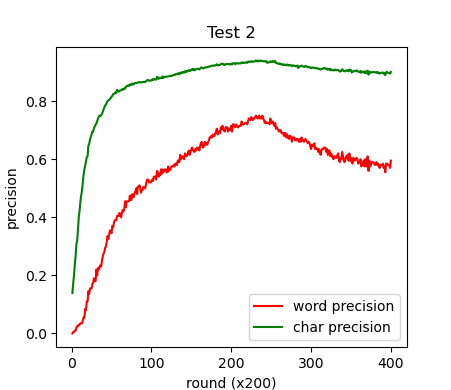
\includegraphics[width=2.8in]{figs/fig1.png}
\end{figure}

\par 最佳模型的性能和cpu上的训练时间为
\begin{table}[H]
    \centering
    \begin{tabular}{cccc}
        \hline 
         & \textbf{单词准确率} & \textbf{字符准确率} \\ 
        \hline 
        \textbf{最佳模型性能} & $75.8\% \pm 1.2\%$ & $94.6\%\pm 0.4\%$ \\ 
        \hline
        \hline
        &\textbf{200个epoch总时间(s)}&\textbf{平均每个epoch的训练时间(s)}\\
        \hline
        \textbf{时间} &$235.5\pm 10.3$ & $1.178\pm0.052$\\
        \hline
    \end{tabular}
\end{table}

\subsubsection{实验3:加入l2正则}
\par 在实验2中出现了明显的过拟合现象,因此考虑在损失函数中加入L2正则化项,正则系数为0.01。
\par 在该设置下,测试集上的单词准确率和字符准确率随训练过程的变化曲线为
\begin{figure}[H]
    \centering
    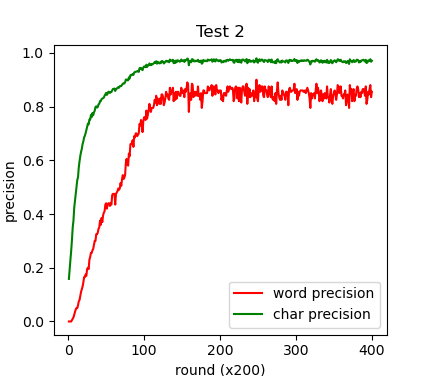
\includegraphics[width=2.8in]{figs/fig2.png}
\end{figure}

\par 最佳模型的性能和cpu上训练时间为
\begin{table}[H]
    \centering
    \begin{tabular}{cccc}
        \hline 
         & \textbf{单词准确率} & \textbf{字符准确率} \\ 
        \hline 
        \textbf{最佳模型性能} & $89.7\% \pm 0.3\%$ & $97.8\%\pm 0.0\%$ \\ 
        \hline
        \hline
        &\textbf{200个epoch总时间(s)}&\textbf{平均每个epoch的训练时间(s)}\\
        \hline
        \textbf{时间} &$227.26\pm 4.3$ & $1.138\pm0.022$\\
        \hline
    \end{tabular}
\end{table}
\par 可见,加入L2正则化后不仅渐进性能提升到了接近90\%,同时也有效避免了过拟合。

\subsubsection{实验4:数据降噪}
\par 可视化图像可以发现,原本的图片中存在大量噪点,对模型性能有较大影响。因此考虑使用average pooling的方式,以2为stride对图片的噪点进行弱化处理(每个像素点的值将被替换为边长为2的视窗内像素点的均值)。
\par 但是由于本身图像的分辨率较低,以stride=2的池化会导致图像“面目全非”。最终结果如下表所示。
\begin{table}[H]
    \centering
    \begin{tabular}{cccc}
        \hline 
         & \textbf{单词准确率} & \textbf{字符准确率} \\ 
        \hline 
        \textbf{最佳模型性能} & $62.5\% \pm 1.5\%$ & $90.3\%\pm 1.3\%$ \\ 
        \hline
        \hline
        &\textbf{200个epoch总时间(s)}&\textbf{平均每个epoch的训练时间(s)}\\
        \hline
        \textbf{时间} &$236.08\pm 8.1$ & $1.180\pm0.041$\\
        \hline
    \end{tabular}
\end{table}


\par \textbf{最终提交的代码为实验3版本,即加入正则化损失后的训练代码。}

\subsection{总结}
\par 以上就是本次实验报告的所有内容,祝老师助教们新年快乐$\sim$


\end{document}